\chapter{Network Models}
\label{chapter:network_models}
A network model comprises atomic models and other network models that are interconnected. Network models can be components of other network models, thereby enabling the construction of very large, multi-level systems. Unlike atomic models, network models do not directly define new dynamic behavior. The dynamics of a network model are determined by the dynamics of its component parts and their interactions. Atomic models define fundamental behaviors; network models define structure. 

\section{Parts of a Network Model}
\label{section:parts_of_a_network_model}
Network models are derived from the abstract \classname{Network} class. This class has two virtual methods: \methodname{route} and \methodname{getComponents}. The \methodname{route} method implements connections between the components of the \classname{Network} model and between those components and the inputs and outputs of the network itself. The \methodname{getComponents} method provides the set of components that constitute the network.

The \methodname{route} method is the primary workhorse of a \classname{Network} model. It realizes three types of connections. The first are connections between components of the network. The second are connections from the network's inputs to the inputs of its component models. The third are connections from the components' outputs to the outputs of the network.

The signature of the \methodname{route} method is
\begin{verbatim}
void route(const X& value, Devs<X>* model, Bag<Event<X> >& r) 
\end{verbatim}
for which the value argument is the object being routed, the model argument is the \classname{Network} or \classname{Atomic} model that originated the event (i.e., the event's source), and the r argument is a bag to be filled with the targets of the event. Each target is described by an \classname{Event} object that carries to pieces of information: a pointer to the model that is the event's target and the object to be delivered to that target.

The simulator uses these \classname{Event} objects in one of three ways, which depending on the relationship between the source of the event and its target. These uses are
\begin{enumerate}
\item If the event's source is a component of the network and the target is the network itself, then the event's value becomes an output from the network.
\item If the event's source is the network and the event's target is a component of the network, then the event's value becomes an input to that component.
\item If the event's source and target are both components of the network, then the event's value becomes an input to the target.
\end{enumerate}
Any other relationship between the source and the target is illegal and will cause the simulator to raise an exception.

The simplest example of how the route method is used converts output from one \classname{Atomic} component of a \classname{Network} into input for another \classname{Atomic} component of the same \classname{Network}. Figure \ref{fig:atomic_to_atomic_coupling} illustrates this case. 
\begin{figure}[ht]
\centering
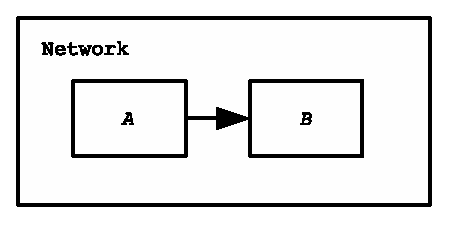
\epsfig{file=network_models_figs/connected_atomic_models.eps}
\caption{Two connected \classname{Atomic} components in a single \classname{Network}.}
\label{fig:atomic_to_atomic_coupling}
\end{figure} 

The simulator begins by invoking the output\_func method of \classname{Atomic} model $A$. Next, the simulator iterates through the elements of $A$'s output bag and calls the \classname{Network}'s route method for each one. The arguments passed to route at each call are
\begin{enumerate}
\item the output object itself, which becomes the value argument,
\item a pointer to $A$, which is the model argument, and
\item an empty \classname{Bag} for holding \classname{Event} objects.
\end{enumerate} 
Two things are done by the \methodname{route} method to cause \classname{Atomic} model $B$ to receive the output object from $A$. First, an \classname{Event} object is created that contains the output object and a pointer to $B$. Second, this \classname{Event} object is inserted into the \classname{Bag} r of receivers of the event. If we suppose, for the sake of illustration, that input and output objects have type int, then the route method for this example is
\begin{verbatim}
void route(const int& value, Devs<int>* model, Bag<Event<int> >& r) {
   if (model == A) {
      Event<int> e(B,value);
      r.insert(e);
   }
}
\end{verbatim}
where $A$ and $B$ are pointers to the respective components. This route method implements the network shown in Fig. \ref{fig:atomic_to_atomic_coupling}.

A more complicated example is the network itself receiving input ultimately destined for one of its atomic components. This can happen, for instance, when the network is a component of another network. Suppose that input to our example network is to become input for \classname{Atomic} model $A$. Figure \ref{fig:eic_atomic_to_atomic_coupling} extends Fig. \ref{fig:atomic_to_atomic_coupling} to include this connection.
\begin{figure}[ht]
\centering
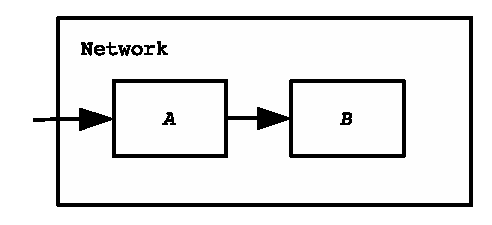
\epsfig{file=network_models_figs/eic_atomic_atomic_coupling.eps}
\caption{Two connected \classname{Atomic} components with external input coupling to component $A$.}
\label{fig:eic_atomic_to_atomic_coupling}
\end{figure} 

When an event appears at the input of the network, the simulator calls the \classname{Network}'s route method with the following arguments:
\begin{enumerate}
\item the input object itself, which becomes the value argument,
\item a pointer to the \classname{Network} that is receiving the event, and
\item an empty \classname{Bag} for holding \classname{Event} objects.
\end{enumerate} 
As before, the \methodname{route} creates an \classname{Event} object that indicates the receiving model and the value of the event. This \classname{Event} object is put into the \classname{Bag} r of receivers. The code below implements the network shown in Fig. \ref{fig:eic_atomic_to_atomic_coupling}; note that the this pointer points to the \classname{Network} itself (i.e., to the network that is receiving the input initially).
\begin{verbatim}
void route(const int& value, Devs<int>* model, Bag<Event<int> >& r) {
   if (model == A) {
       Event<int> e(B,value);
       r.insert(e);
   }
   else if (model == this) {
       Event<int> e(A,value);
       r.insert(e);
   }
}
\end{verbatim}
\begin{figure}[ht]
\centering
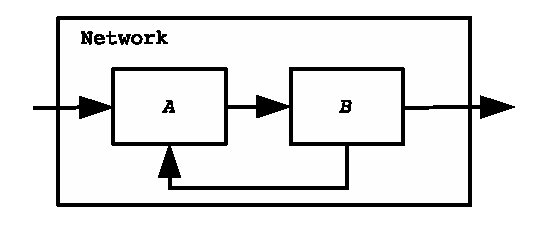
\epsfig{file=network_models_figs/big_coupled.eps}
\caption{A two component network model with external input, external output, and internal coupling.}
\label{fig:big_coupling}
\end{figure} 

For a complete example, the network is extended again, as shown in Fig. \ref{fig:eic_atomic_to_atomic_coupling}, to include two more connections: a connection from the output of model $B$ to the output of the network and a feedback connection from $B$ to $A$. This configuration is shown in Fig. \ref{fig:big_coupling}. This new connection requires an additional case in the route method. This case checks for output from $B$ and, if such an output is found, directs it to both $A$ and the network itself. A \classname{Event} object is created for each target and added to the \classname{Bag} r of receivers: one of these \classname{Event}s results in an input to $A$ and the other in an output from the network. Here is the implementation.
\begin{verbatim}
void route(const int& value, Devs<int>* model, Bag<Event<int> >& r) {
   if (model == A) {
        Event<int> e(B,value);
        r.insert(e);
    }
    else if (model == this) {
        Event<int> e(A,value);
        r.insert(e);
    }
    else if (model == B) {
        Event<int> e1(this,value);
        Event<int> e2(A,value);
        r.insert(e1);
        r.insert(e2);
    }
}
\end{verbatim}

The getComponents method is the other virtual method that must be implemented by a \classname{Network}. The simulator passes to this method an empty \classname{Set} of pointers to models, and this must be filled with the network's components. The signature of the getComponents method is
\begin{verbatim}
void getComponents(Set<Devs<X>*>& c) 
\end{verbatim}
where c is the set to be filled. There isn't much else to say about this method. The code below shows how it is implemented for the two component network shown in Fig. \ref{fig:big_coupling}; this code, of course, also works for the networks shown in Figs. \ref{fig:eic_atomic_to_atomic_coupling} and \ref{fig:atomic_to_atomic_coupling}.
\begin{verbatim}
void getComponents(Set<Devs<int>*>& c) { 
   c.insert(A);
   c.insert(B);
}
\end{verbatim}

There are just three other items to mention in relation to \classname{Network} models. First, components cannot be connected to themselves. This means that direct feedback loops and connections direct through a network model are illegal. The former can always be replaced with an internal event an the latter by simply bypassing the network (which won't do anything with the input in any event). These two cases are illustrated in Fig. \ref{fig:bad_coupling}. Second, direct coupling can only occur between components belonging to the same network, and every component must belong to, at most, one network. Third, the \methodname{route} method is allowed to modify an output before sending it along; this can be useful in some cases.
\begin{figure}[ht]
\centering
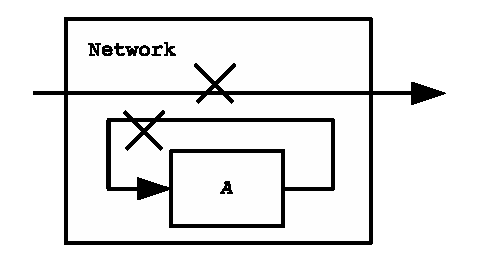
\epsfig{file=network_models_figs/bad_couplings.eps}
\caption{Illegal coupling in a \classname{Network} model.}
\label{fig:bad_coupling}
\end{figure}

\section{Simulating a Network Model}
Each iteration of the simulator has four phases: 1) advance the simulation clock to the time of the next event, 2) compute the outputs from atomic models that will change state (i.e., how will undergo an internal or confluent event) and convert these outputs into inputs for other models, 3) calculate the next state of each model with events to process, and 4) cleanup garbage left over from the output calculations. These four phase are repeated until the time of the next event is at infinity (i.e., DBL\_MAX) or you decide to stop the simulation. 

Conveniently, there are no special rules for simulating networks of network models. The simulator considers the entire collection of atomic models when determining the next event time; output from atomic models are recursively routed to their atomic destinations; and the state transitions and garbage collection are performed over the complete set of active atomic components. Hierarchies of network models are a convenient organizing tool for the modeler, but the simulator treats (via its recursive routing of events) the multi-level network as a flat structure.

Algorithm \ref{alg:coupled_model} sketches the simulation procedure. Note that the procedure for simulating atomic models (see section \ref{section:atomic_models}) is embedded in the procedure for simulating network models. The rules for atomic models do not change in any way; each atomic model sees a sequence of input events and produces a sequence of output events just as before. The only difference here is that the input events are created by other atomic models, and so the input sequence for each atomic model is constructed as the simulation progresses.
\begin{algorithm}
\begin{algorithmic}
\STATE Initialize the state of every \classname{Atomic} model 
\STATE Set the time of last event $t_{l,i}$ of every \classname{Atomic} model $i$ to $0$
\STATE Set the simulation time $t$ to $0$
\WHILE {The smallest time of next event for the \classname{Atomic} models is less than DBL\_MAX}
   \STATE Set $t$ to the smallest time of next event for the \classname{Atomic} models
   \STATE Find the set of \classname{Atomic} models whose next event time is equal to $t$. These are the imminent models.
   \STATE Get the output of each imminent model by calling its \methodname{output\_func}
   \
   \STATE Convert output from imminent models to input for other models using the \classname{Network} models \methodname{route} methods (do this recursively if the network has more than one level)
   \FOR{each \classname{Atomic} model $i$ that is imminent or has input}
      \IF {$i$ is an imminent model and it does not have input}
         \STATE Compute the next model state with delta\_int()
      \ELSIF {$i$ is an imminent and it has input}
         \STATE Compute the next model state with delta\_conf(xb), where xb is the model input
      \ELSIF {$i$ is not an imminent model and it has input}
         \STATE Compute the next model state with delta\_ext($t-t_{l,i}$,xb), where xb is the model input
      \ENDIF
      \STATE Set $t_{l,i}$ to $t$
   \ENDFOR
\ENDWHILE
\end{algorithmic}
\caption{The simulation procedure for a network model.}
\label{alg:coupled_model}
\end{algorithm}

\section{A complete example of a network model}
I'll use the \adevs\ \classname{SimpleDigraph} class to illustrate the process of building a network model. The \classname{SimpleDigraph} models a network of components whose connections are represented with a directed graph. If, for example, component $A$ is connected to component $B$, then all output events generated by $A$ become input events to $B$.

The \classname{SimpleDigraph} has two methods for building a network. The \methodname{add} method takes an \classname{Atomic} or \classname{Network} model and adds it to the set of components. The \methodname{couple} method accepts a pair of components and connects the first to the second. Below is the class definition for the model; note that is has a template parameter for setting its input and output type. The \classname{Network}, \classname{Devs}, \classname{Bag}, and \classname{Set} are in the adevs namespace, and \mbox{adevs::} must precede them unless the \classname{SimpleDigraph} is itself in the adevs namespace (which, in this case, it is). 
\begin{verbatim}
template <class VALUE> class SimpleDigraph: public Network<VALUE> { 
   public:
      /// A component of the SimpleDigraph model
      typedef Devs<VALUE> Component;

      /// Construct a network with no components
      SimpleDigraph():Network<VALUE>(){}
      /// Add a model to the network.
      void add(Component* model);
      /// Couple the source model to the destination model  
      void couple(Component* src, Component* dst);
      /// Assigns the model component set to c
      void getComponents(Set<Component*>& c);
      /// Use the coupling information to route an event
      void route(const VALUE& x, Component* model, Bag<Event<VALUE> >& r);
      /// The destructor destroys all of the component models
      ~SimpleDigraph();

   private:   
      // Component model set
      Set<Component*> models;
      // Coupling information
      std::map<Component*,Bag<Component*> > graph;
};
\end{verbatim}
The \classname{SimpleDigraph} has two member variables. The first is a set of pointers to the components of the network; these are stored in the \classname{Set} models. The components can be \classname{Atomic} objects, \classname{Network} objects, or both. The \classname{SimpleDigraph} components are the nodes of the directed graph. The second member variable is a STL map that contains the network's links, or edges; these are stored in the \classname{map} graph.

The \classname{SimpleGraph} has four methods beyond the required route and getComponents. One of these is the constructor, which creates an empty network. The other is the destructor, which deletes all of the network's components. The others are add and couple.

The add method does three things. First, it checks that the network is not being added to itself; this is illegal and would cause no end of trouble for the simulator. Next, it adds the new component to its set of components. Last, the \classname{SimpleNetwork} sets the component's parent. The last step is needed so that the simulator can climb up and down the model tree. If it is omitted then the routing of events is likely fail. Here is the implementation of the \methodname{add} method.
\begin{verbatim}
template <class VALUE> 
void SimpleDigraph<VALUE>::add(Component* model) {
   assert(model != this);
   models.insert(model);
   model->setParent(this);
}
\end{verbatim}

The couple method does two things, but one of them is somewhat superfluous. First, it adds the source (src) and destination (dst) models to the set of components. We could simply have required that the user call the add method before using the couple method, but adding the components here doesn't hurt and might prevent an error. The second step is essential; the method adds the \mbox{src $\rightarrow$ dst} link to the graph. Notice that the \methodname{SimpleDigraph} itself is a node in the network (but it is not in the set of components!): components that are connected to the network cause network outputs. Similarly, connecting the network to a component cause input to the network to become input to that component. Here is the implementation of the couple method.
\begin{verbatim}
template <class VALUE>
void SimpleDigraph<VALUE>::couple(Component* src, Component* dst) { 
   if (src != this) add(src);
   if (dst != this) add(dst);
   graph[src].insert(dst);
}
\end{verbatim}

Of the two required methods, route is the more complicated. The arguments to route are an object that is the value to be routed, the network element (i.e., either the \classname{SimpleDigraph} or one of its components) that created that object, and the \classname{Bag} to be filled with \classname{Event} objects that indicate the object's receivers. The method begins by finding the collection of components that are connected to the source of the event. Next, it iterates through this collection and for each receiver adds an \classname{Event} to the \classname{Bag} of receivers. When this is done the method returns. The implementation is below.
\begin{verbatim}
template <class VALUE>
void SimpleDigraph<VALUE>::route(const VALUE& x, Component* model,Bag<Event<VALUE> >& r) {
   // Find the list of target models and ports
   typename std::map<Component*,Bag<Component*> >::iterator graph_iter;
   graph_iter = graph.find(model);
   // If no target, just return
   if (graph_iter == graph.end()) return;
   // Otherwise, add the targets to the event bag
   Event<VALUE> event;
   typename Bag<Component*>::iterator node_iter;
   for (node_iter = (*graph_iter).second.begin();
      node_iter != (*graph_iter).second.end(); node_iter++) {
      event.model = *node_iter;
      event.value = x;
      r.insert(event);
   }
}
\end{verbatim}

The second required method, getComponents, is trivial. If we had used some collection other than an \adevs\ \classname{Set} to store the components, then the method would have needed to explicitly insert every component model into the \classname{Set} c. But because the sets models and c are both \classname{Set} objects, and the \classname{Set} has an assignment operator, a simple call to that operator is sufficient.
\begin{verbatim}
template <class VALUE>
void SimpleDigraph<VALUE>::getComponents(Set<Component*>& c) {
   c = models;
}
\end{verbatim}

The constructor and the destructor complete the class. The constructor implementation appears in the class definition; it only calls the superclass constructor. The destructor deletes the component models. Its implementation is shown below.
\begin{verbatim}
template <class VALUE>
SimpleDigraph<VALUE>::~SimpleDigraph() {
   typename Set<Component*>::iterator i;
   for (i = models.begin(); i != models.end(); i++) {
      delete *i;
   }
}
\end{verbatim}
 
\section{Digraph Models}
\label{section:digraph_models}
This section introduces the \classname{Digraph} model, which is part of the \adevs\ simulation library. The \classname{Digraph} is a tool for building network models based on, or described by, a block diagram. The model of the convenience store, developed in section \ref{chapter:intro}, was our first example of a \classname{Digraph} model. The code used to construct the convenience store model (without the \classname{Observer}) is shown below. The block diagram that corresponds to this code snippet is shown in Fig. \ref{fig:two_component_diagram}.
\begin{verbatim}
// Create a digraph model whose components use PortValue<Customer*>
// objects as input and output objects.
adevs::Digraph<Customer*> store;
// Create and add the component models
Clerk* clrk = new Clerk();
Generator* genr = new Generator(argv[1]);
store.add(clrk);
store.add(genr);
// Couple the components
store.couple(genr,genr->arrive,clrk,clrk->arrive);
\end{verbatim}
\begin{figure}[ht]
\centering
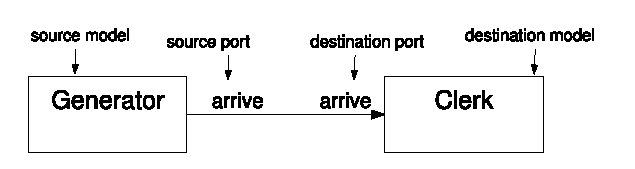
\epsfig{file=network_models_figs/two_component_model.eps}
\caption{A \classname{Digraph} model with two components.}
\label{fig:two_component_diagram}
\end{figure}

The components of a \classname{Digraph} must use \classname{adevs::PortValue} objects for their input and output type.  The \classname{Digraph} is a template class with two template parameters. The first parameter is the type of object used for a value in the \classname{PortValue} objects. The second parameter is the type of object used for a port in the \classname{PortValue} objects. The port parameter is of type 'int' by default.

For the modeler, the \classname{Digraph} has two primary methods. The add method is used to add components to the network; the argument to the add method is just the model to be included in the network. The couple method is used to connect components of the network. The first two arguments to the couple method are the source model and source port. The second two arguments are the destination model and the destination port.
 
The effect of coupling a source model to a destination model is that output produced by the source model on the source port appears as input to the destination model on the destination port. To illustrate this, consider the output function of the \classname{Generator} model that is shown in Fig. \ref{fig:two_component_diagram}.
\begin{verbatim}
void Generator::output_func(Bag<IO_Type>& yb)
{
    // First customer in the list is produced as output
    IO_Type output(arrive,arrivals.front());
    yb.insert(output);
}
\end{verbatim}

This output function places an output value of type `Customer*' on the ``arrive'' output port of the \classname{Generator}; recall that 'IO\_Type' is a typedef for `PortValue<Customer*>'. A corresponding \classname{PortValue} object appears in the input bag of the \classname{Clerk}. The value attribute of the \classname{PortValue} object received by the clerk points to the \classname{Customer} object created by the \classname{Generator}, and the port is the \classname{Clerk}'s ``arrive" port.

The components for the network need not consist only of \classname{Atomic} models; the \classname{Digraph} can also have other \classname{Network} models as its components. For instance, suppose that we want to model a convenience store that has two clerks. When customers are ready to pay their bill, they enter the shortest line. To build this model, we reuse the \classname{Clerk}, \classname{Generator}, and \classname{Observer} models that were introduced in section \ref{chapter:intro}, and add an additional model for the process of customers selecting a checkout line.

The header and source code for the model of the line-selection process is shown below. This model has two output ports, one for each line, and there are three input ports. One input port accepts new customers. The others are used to track the number of number of customers departing each line: a customer departing either clerk generates an event on the appropriate input port. In this way, the model is able to track the number of customers in each line and assign new customers to the shortest one. With this information, the state transition and output functions are (I hope) self explanatory. Here is the class definition
\begin{verbatim}
#include "adevs.h"
#include "Customer.h"
#include <list>

// Number of lines to consider.
#define NUM_LINES 2

class Decision: public adevs::Atomic<IO_Type>
{
    public:
        /// Constructor.
        Decision();
        /// Internal transition function.
        void delta_int();
        /// External transition function.
        void delta_ext(double e, const adevs::Bag<IO_Type>& x);
        /// Confluent transition function.
        void delta_conf(const adevs::Bag<IO_Type>& x);
        /// Output function.  
        void output_func(adevs::Bag<IO_Type>& y);
        /// Time advance function.
        double ta();
        /// Output value garbage collection.
        void gc_output(adevs::Bag<IO_Type>& g);
        /// Destructor.
        ~Decision();
        /// Input port that receives new customers
        static const int decide;
        /// Input ports that receive customers leaving the two lines
        static const int departures[NUM_LINES];
        /// Output ports that produce customers for the two lines
        static const int arrive[NUM_LINES];

    private:
        /// Lengths of the two lines
        int line_length[NUM_LINES];
        /// List of deciding customers and their decision.
        std::list<std::pair<int,Customer*> > deciding;
        /// Delete all waiting customers and clear the list.
        void clear_deciders();
        /// Returns the arrive port associated with the shortest line
        int find_shortest_line();
};
\end{verbatim}
and here is the implementation
\begin{verbatim}
#include "Decision.h"
#include <iostream>
using namespace std;
using namespace adevs;

// Assign identifiers to ports.  Assumes NUM_LINES = 2.
// The numbers are selected to allow indexing into the
// line length and port number arrays.
const int Decision::departures[NUM_LINES] = { 0, 1 };
const int Decision::arrive[NUM_LINES] = { 0, 1 };
// Inport port for arriving customer that need to make a decision
const int Decision::decide = NUM_LINES;

Decision::Decision():
Atomic<IO_Type>()
{
    // Set the initial line lengths to zero
    for (int i = 0; i < NUM_LINES; i++)
    {
        line_length[i] = 0;
    }
}

void Decision::delta_int()
{
    // Move out all of the deciders
    deciding.clear();
}

void Decision::delta_ext(double e, const Bag<IO_Type>& x)
{
    // Assign new arrivals to a line and update the line length
    Bag<IO_Type>::const_iterator iter = x.begin();
    for (; iter != x.end(); iter++)
    {
        if ((*iter).port == decide)
        {
            int line_choice = find_shortest_line();
            Customer* customer = new Customer(*((*iter).value));
            pair<int,Customer*> p(line_choice,customer);
            deciding.push_back(p);
            line_length[p.first]++;
        }
    }
    // Decrement the length of lines that had customers leave
    for (int i = 0; i < NUM_LINES; i++)
    {
        iter = x.begin();
        for (; iter != x.end(); iter++)
        {
            if ((*iter).port < NUM_LINES)
            {
                line_length[(*iter).port]--;
            }
        }
    }
}

void Decision::delta_conf(const Bag<IO_Type>& x)
{
    delta_int();
    delta_ext(0.0,x);
}

double Decision::ta()
{
    // If there are customers getting into line, then produce output
    // immediately.
    if (!deciding.empty())
    {
        return 0.0;
    }
    // Otherwise, wait for another customer
    else
    {
        return DBL_MAX;
    }
}
        
void Decision::output_func(Bag<IO_Type>& y)
{
    // Send all customers to their lines
    list<pair<int,Customer*> >::iterator i = deciding.begin();
    for (; i != deciding.end(); i++)
    {
        IO_Type event((*i).first,(*i).second);
        y.insert(event);
    }
}

void Decision::gc_output(Bag<IO_Type>& g)
{
    Bag<IO_Type>::iterator iter = g.begin();
    for (; iter != g.end(); iter++)
    {
        delete (*iter).value;
    }
}

Decision::~Decision()
{
    clear_deciders();
}

void Decision::clear_deciders()
{
    list<pair<int,Customer*> >::iterator i = deciding.begin();
    for (; i != deciding.end(); i++)
    {
        delete (*i).second;
    }
    deciding.clear();
}

int Decision::find_shortest_line()
{
    int shortest = 0;
    for (int i = 0; i < NUM_LINES; i++)
    {
        if (line_length[shortest] > line_length[i])
        {
            shortest = i;
        }
    }
    return shortest;
}
\end{verbatim}

The block diagram of the store with multiple clerks is shown in Fig. \ref{fig:multi_clerk_diagram}. The external interface for this block diagram model is identical to that of the clerk models (i.e., it has the same inputs and outputs as the \classname{Clerk} and \classname{Clerk2} models), and we can therefore use the generator and observer models to conduct the same experiments as before. The external ``arrive" input of the multi-clerk model is connected to the ``decide" input of the \classname{Decision} model. The ``depart" output ports of each of the \classname{Clerk} models is connected to the external ``arrive" output port of the multi-clerk model. The \classname{Decision} model has two output ports, each one producing customers for a distinct clerk. These output ports are coupled to the ``arrive" port of the appropriate clerk. The \classname{Clerk}'s ``depart" output ports are then coupled to the appropriate ``departures" port of the decision model.
\begin{figure}[ht]
\centering
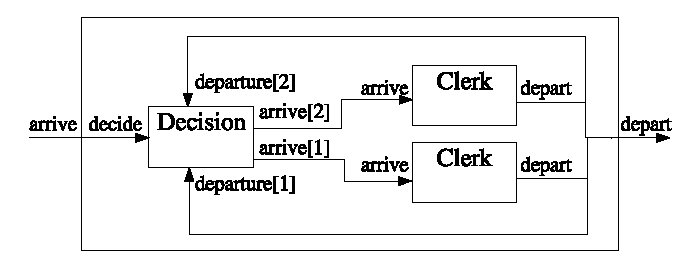
\epsfig{file=network_models_figs/multi_clerk_diagram.eps}
\caption{Component models and their interconnections in the multi-clerk convenience store model.}
\label{fig:multi_clerk_diagram}
\end{figure}    

The multi-clerk model is implemented by deriving a new class from \classname{Digraph}. The constructor of the new class creates and adds the component models and establishes their interconnections. Here is the header file for this new multi-clerk model.
\begin{verbatim}
#include "adevs.h"
#include "Clerk.h"
#include "Decision.h"

/**
A model of a store with multiple clerks and a "shortest line"
decision process for customers.
*/
class MultiClerk: public adevs::Digraph<Customer*>
{
    public:
        // Model input port
        static const int arrive;
        // Model output port
        static const int depart;
        // Constructor.
        MultiClerk();
        // Destructor.
        ~MultiClerk();
};
\end{verbatim}
And here is the source file
\begin{verbatim}
#include "MultiClerk.h"
using namespace std;
using namespace adevs;

// Assign identifiers to I/O ports
const int MultiClerk::arrive = 0;
const int MultiClerk::depart = 1;

MultiClerk::MultiClerk():
Digraph<Customer*>()
{
    // Create and add component models
    Decision* d = new Decision();
    add(d);
    Clerk* c[NUM_LINES];
    for (int i = 0; i < NUM_LINES; i++)
    {
        c[i] = new Clerk();
        add(c[i]);
    }
    // Create model connections
    couple(this,this->arrive,d,d->decide);
    for (int i = 0; i < NUM_LINES; i++)
    {
        couple(d,d->arrive[i],c[i],c[i]->arrive);
        couple(c[i],c[i]->depart,d,d->departures[i]);
        couple(c[i],c[i]->depart,this,this->depart);
    }
}

MultiClerk::~MultiClerk()
{
}
\end{verbatim}
Notice that the \classname{MultiClerk} destructor does not delete its component models. This is because the components are adopted by the base class when they are added using the \classname{Digraph}'s add method. Consequently, the component models are deleted by the base class destructor, rather than the destructor of the derived class.

\section{Cell Space Models}
A cell space model is a collection of atomic and network models arrange in a regular grid and with each model connected to its neighboring models. Conway's Game of Life is a classic example of a cell space model that can be described very nicely as a discrete event system. The game is played on a flat board divided into regular cells much like a checkerboard. Each cell has a neighborhood that consists of its eight adjacent cells: above, below, left, right, and the four corners. A cell can be dead or alive, and the switch from dead to alive and vice versa occurs according to two rules:
\begin{enumerate}
\item (Death rule). If a cell is alive and it has less than two or more than three living neighbors then the cell dies.
\item (Rebirth rule). If a cell is dead and it has three three living neighbors then the cell is reborn.
\end{enumerate}

Our implementation of the Game of Life has two parts: the atomic models that implement the individual cells and the \classname{CellSpace} that contains the cells. The \classname{CellSpace} is a type of \classname{Network}, and its components exchange \classname{CellEvent} objects that have four attributes: the x, y, and z coordinates of the target cell (the cell space can have three dimensions; the game of life uses just two) and the object to deliver to that target. The \classname{CellEvent} class is a template class whose template argument sets the type of object that the event delivers. The size of the \classname{CellSpace} is determined when the \classname{CellSpace} object is created, and it has methods for adding and retrieving cells by location. 

The \classname{Atomic} cells in our Game of Life have two state variables: one is the dead or alive status of the cell and the other is its count of living neighbors. Two methods are implemented to test the death and rebirth rules, and the cell sets its time advance to 1 whenever a rule is satisfied. The cell's output is its new dead or alive state. External events update the cell's count of living neighbors. In order to produce properly targeted \classname{CellEvent}s, each cell also keeps track of its own location in the cell space. In the example code, the cell space is rendered graphically using OpenGL, but I'll omit that part. Here is the abbreviated header file for our Game of Life cell.
\begin{verbatim}
/// Possible cell phases
typedef enum { Dead, Alive } Phase;
/// IO type for a cell
typedef adevs::CellEvent<Phase> CellEvent;

/// A cell in the Game of Life.  
class Cell: public adevs::Atomic<CellEvent> {
   public:
      /**
      Create a cell and set the initial state.
      The width and height fields are used to determine if a
      cell is an edge cell.  The last phase pointer is used to
      visualize the cell space.
      */
      Cell(long int x, long int y, long int width, long int height, 
      Phase phase, short int nalive, Phase* vis_phase = NULL);

      ... Required Adevs methods and destructor ...

   private:   
      // location of the cell in the 2D space
      long int x, y;
      // dimensions of the 2D space
      static long int w, h;
      // Current cell phase
      Phase phase;
      // number of living neighbors.
      short int nalive;
      // Output variable for visualization
      Phase* vis_phase;

      // Returns true if the cell will be born
      bool check_born_rule() const {
         return (phase == Dead && nalive == 3);
      }
      // Return true if the cell will die
      bool check_death_rule() const {
         return (phase == Alive && (nalive < 2 || nalive > 3));
      }
};
\end{verbatim}

The template argument supplied to the base \classname{Atomic} class is a \classname{CellEvent} whose value attribute has the type \classname{Phase}. The check\_born\_rule method tests the rebirth condition and the check\_death\_rule method tests the death condition. The appropriate rule, as determined by the cell's dead or alive status, is used in the time advance, output, and internal transition methods (i.e., if the cell is dead then check the rebirth rule; if alive, check the death rule). The number of living cells is updated by the cell's \methodname{delta\_ext} method when neighboring cells report a change in their status. Here are the \classname{Cell}'s method implementations.
\begin{verbatim}
Cell::Cell(long int x, long int y, long int w, long int h, 
Phase phase, short int nalive, Phase* vis_phase):
adevs::Atomic<CellEvent>(),x(x),y(y),phase(phase),nalive(nalive),vis_phase(vis_phase) {
   // Set the global cellspace dimensions
   Cell::w = w; Cell::h = h;
   // Set the initial visualization value
   if (vis_phase != NULL) *vis_phase = phase;
}

double Cell::ta() {
   // If a phase change should occur then change state 
   if (check_death_rule() || check_born_rule()) return 1.0;
   // Otherwise, do nothing
   return DBL_MAX;
}

void Cell::delta_int() { 
   // Change the cell state if necessary
   if (check_death_rule()) phase = Dead;
   else if (check_born_rule()) phase = Alive;
}

void Cell::delta_ext(double e, const adevs::Bag<CellEvent>& xb) {
   // Update the living neighbor count 
   adevs::Bag<CellEvent>::const_iterator iter;
   for (iter = xb.begin(); iter != xb.end(); iter++) {
      if ((*iter).value == Dead) nalive--;
      else nalive++;
   }
}

void Cell::delta_conf(const adevs::Bag<CellEvent>& xb) { 
   delta_int();
   delta_ext(0.0,xb);
}

void Cell::output_func(adevs::Bag<CellEvent>& yb) { 
   CellEvent e;
   // Assume we are dying
   e.value = Dead;
   // Check in case this in not true
   if (check_born_rule()) e.value = Alive;
   // Set the visualization value
   if (vis_phase != NULL) *vis_phase = e.value;
   // Generate an event for each neighbor
   for (long int dx = -1; dx <= 1; dx++) {
      for (long int dy = -1; dy <= 1; dy++) {
         e.x = (x+dx)%w;
         e.y = (y+dy)%h;
         if (e.x < 0) e.x = w-1;
         if (e.y < 0) e.y = h-1;
         // Don't send to self
         if (e.x != x || e.y != y)
            yb.insert(e);
      }
   }
}
\end{verbatim}
The \methodname{output\_func} method shows how a cell sends messages to its neighbors. The double for loop creates a \classname{CellEvent} targeted at each adjacent cell. The location of the target cell is written to the x, y, and z attributes of the \classname{CellEvent} object. Just like arrays, the locations can range from zero to the cell space's size minus one. The \classname{CellSpace} routes the \classname{CellEvent}s to their targets. However, if the target of the \classname{CellEvent} is outside of the cell space, then the \classname{CellSpace} itself will produce the \classname{CellEvent} as an output.

The remainder of the simulation program looks very much like the simulation programs that we've seen so far (except for some OpenGL specific code, omitted here, that is used to display the cells). A \classname{CellSpace} object is created and we add the cells to it. Then a \classname{Simulator} object is create and a pointer to the \classname{CellSpace} is passed to the \classname{Simulator}'s constructor. Last, we execute events until our stopping criteria is met. The execution part is already familiar, so let's just focus on creating the \classname{CellSpace}. Here is the code snippet that performs the construction.
\begin{verbatim}
// Create the cellspace model
cell_space = new adevs::CellSpace<Phase>(WIDTH,HEIGHT);
for (int x = 0; x < WIDTH; x++) {
   for (int y = 0; y < HEIGHT; y++) {
       // Count the living neighbors
       short int nalive = count_living_cells(x,y);
       // The 2D phase array contains the initial Dead/Alive state of each cell
       cell_space->add(new Cell(x,y,WIDTH,HEIGHT,phase[x][y],nalive,&(phase[x][y])),x,y);
   }
}
\end{verbatim}
Just as with the \classname{Digraph} class, the \classname{CellSpace} template argument determines the value type for the \classname{CellEvent}s used as input and output by the component models. The \classname{CellSpace} constructor sets the dimensions of the space. Every \classname{CellSpace} is three dimensional, and the constructor accepts three arguments that set its x, y, and z dimensions; omitted arguments default to 1. The constructor signature is
\begin{verbatim}
CellSpace(long int width, long int height = 1, long int depth = 1)
\end{verbatim}

Components are added to the cellspace with the \methodname{add} method. This method places a component at a specific x,y,z location. Its signature is
\begin{verbatim}
void add(Cell* model, long int x, long int y = 0, long int z = 0)
\end{verbatim}
where \classname{Cell} is a \classname{Devs} (atomic or network) by the type definition
\begin{verbatim}
typedef Devs<CellEvent<X> > Cell;
\end{verbatim}
Also like the \classname{Digraph}, the \classname{CellSpace} deletes its components when it is deleted.

The \classname{CellSpace} has five other methods for retrieving cells and for getting the dimensionality of the cell space. These are more or less self-explanatory; the signatures are shown below.
\begin{verbatim}
const Cell* getModel(long int x, long int y = 0, long int z = 0) const;
Cell* getModel(long int x, long int y = 0, long int z = 0);
long int getWidth() const;
long int getHeight() const;
long int getDepth() const;
\end{verbatim}

The Game of Life produces a surprising number of clearly recognizable patterns. Some of these patterns are fixed and unchanging; others oscillate, cycling through a set of patterns that always repeats itself; others seem to crawl or fly. One common pattern is the Block, which is shown in Fig. \ref{fig:gol_block}. Our discrete event implementation of the Game of Life doesn't do any work when simulating a Block. None of the cells in a Block change in any way: their phases are constant and so are their neighbor counts.
\begin{figure}[ht]
\centering
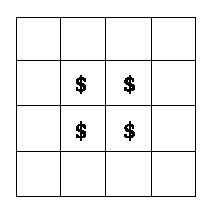
\epsfig{file=network_models_figs/block_pattern.eps}
\caption{The Block.}
\label{fig:gol_block}
\end{figure}
\begin{figure}[ht]
\centering
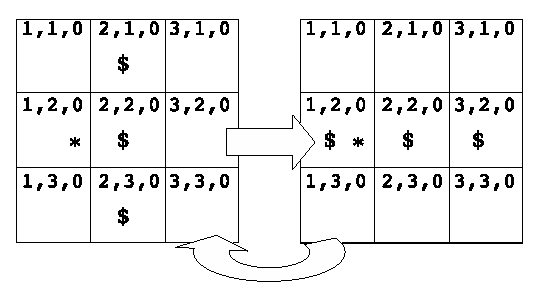
\epsfig{file=network_models_figs/blinker.eps}
\caption{The Blinker. The input, output, and state transitions for the cell marked with a * are shown in Table \ref{tab:blinker_cell_activity}. The address of each cell is shown in its upper left corner. Living cells are indicated with a \$.}
\label{fig:gol_blinker}
\end{figure}
The Blinker shown in Fig. \ref{fig:gol_blinker} is more interesting. This oscillating pattern has just two stages: a vertical and a horizontal. Table \ref{tab:blinker_cell_activity} shows the input, output, and state transitions that are computed for the cell marked with a * in Fig. \ref{fig:gol_blinker}. Just like the pattern it is a part of, the cells oscillates between two different states. 
\begin{table}[ht]
\centering
\begin{tabular}{|l|l|l|l|}
\hline Time & State      & Input & Output to all neighbors\\ \hline
0 & (dead,3) & No input & No Output \\ \hline 
1 & (alive,1) & (dead,2,1,0) \ (dead,2,3,0) & alive \\ \hline 
2 & (dead,1) & (alive,2,1,0) \ (alive,2,3,0) & dead \\ \hline
\end{tabular}
\caption{State, input, and output trajectory for the cell marked with * in Fig. \ref{fig:gol_blinker}.}
\label{tab:blinker_cell_activity}
\end{table}

The confluent transition function plays a major role in the Blinker simulation. Most of the rows in Table \ref{tab:blinker_cell_activity} (all but the first row, in fact) have simultaneous input and output, which means that an internal and external event coincide. Consequently, the next state of the cell is determined by its \methodname{delta\_conf} method. It is also important that the input and output bags carry multiple values. The external transition function (which is used in defining the confluent transition function) must be able to compute the number of living neighbors before determining its next state. If input events were provided one at a time (e.g., if the input bag were replaced by a single input event), then our discrete event Game of Life would be much more difficult to implement.
